% =========================================================================
% CAPITOLO 6: INTRODUZIONE, DATASET E PROCESSO DI ETL (TRANSFERMARKT)
% =========================================================================
\section{Analisi delle serie storiche sul mercato calcistico: introduzione e dataset}

Nel corso degli ultimi quindici anni l'industria calcistica europea ha attraversato una trasformazione economica profonda, evolvendo da settore prevalentemente sportivo a mercato finanziario globale caratterizzato da flussi di capitale miliardari, cicli stagionali regolari e forte sensibilità agli shock macroeconomici esterni. L'espansione dei diritti televisivi internazionali, l'ingresso di fondi sovrani e grandi gruppi di investimento nella proprietà dei club e l'inflazione strutturale dei costi di trasferimento hanno progressivamente ridefinito il valore patrimoniale delle rose dei principali campionati europei. In questo scenario, lo studio dell'evoluzione temporale del valore economico dei calciatori e dei volumi di spesa generati nelle sessioni di calciomercato rappresenta un banco di prova ideale per l'applicazione delle metodologie di analisi e previsione delle serie storiche.

A differenza dei mercati azionari tradizionali, dove il prezzo di un titolo viene battuto in modo continuo durante le sedute di borsa, il mercato calcistico presenta una struttura informativa composita: le valutazioni economiche dei singoli atleti vengono aggiornate periodicamente dagli analisti di mercato in finestre prestabilite durante la stagione sportiva, mentre le transazioni monetarie effettive e gli spostamenti dei giocatori tra i club si concentrano nelle due sessioni ufficiali di calciomercato (quella invernale di gennaio e quella estiva tra luglio e agosto). La seconda parte del presente elaborato si pone l'obiettivo di ricostruire, esplorare e modellare matematicamente la serie storica mensile del valore di mercato delle rose dei cinque maggiori campionati europei (Serie A, Premier League, LaLiga, Bundesliga e Ligue 1), affiancando all'analisi aggregata europea un approfondimento specifico dedicato al campionato italiano di Serie A.

Il percorso metodologico sviluppato nei capitoli successivi si articola in quattro fasi consequenziali: la progettazione di una pipeline di ingegneria dei dati capace di trasformare le tabelle relazionali grezze in una serie storica mensile regolare e priva di discontinuità artificiali; l'analisi esplorativa dei dati e lo studio quantitativo dei grandi shock storici che hanno colpito il settore (dall'esplosione inflattiva del 2017 legata al trasferimento record di Neymar fino alla contrazione pandemica del 2020 e al successivo rimbalzo post-pandemico); la decomposizione stagionale e la verifica formale delle proprietà di stazionarietà e autocorrelazione temporale; infine, l'addestramento e il confronto critico di modelli previsionali di complessità crescente, dai modelli autoregressivi classici fino ai modelli stagionali con variabili esogene (dove il volume di spesa e il numero di trasferimenti del calciomercato vengono impiegati come predittori esterni della dinamica del valore delle rose).

\subsection{Struttura del dataset relazionale di Transfermarkt}

La base informativa utilizzata per lo studio proviene dal repository pubblico \textit{Football Data from Transfermarkt} distribuito sulla piattaforma Kaggle. A differenza di un dataset nativo di serie storiche, la fonte originale è organizzata come un database relazionale composto da dodici tabelle distinte in formato \texttt{.csv}, che registrano l'anagrafica dei campionati, dei club e dei giocatori insieme allo storico granulare delle partite disputate, delle presenze individuali, dei trasferimenti ufficiali e delle valutazioni di mercato.

Per la costruzione della serie storica del valore patrimoniale delle rose e dei flussi di calciomercato, l'attenzione si è concentrata sulle cinque tabelle fondamentali riassunte nella Tabella \ref{tab:tabelle_transfermarkt}. La tabella centrale è costituita dal file \texttt{player\_valuations.csv}, che raccoglie 656.301 osservazioni storiche relative alle stime di valore di mercato espresse in euro (\texttt{market\_value\_in\_eur}) attribuite a ciascun calciatore identificato tramite la chiave primaria \texttt{player\_id} in una determinata data (\texttt{date}). A questa si affianca il file \texttt{transfers.csv}, contenente 175.165 record di trasferimento che documentano per ogni operazione la data esatta (\texttt{transfer\_date}), il club di provenienza (\texttt{from\_club\_id}), il club di destinazione (\texttt{to\_club\_id}), il corrispettivo economico pagato per il cartellino (\texttt{transfer\_fee}) e la valutazione del giocatore al momento del passaggio.

\begin{table}[H]
\centering
\caption{Riepilogo delle tabelle relazionali del dataset di Transfermarkt utilizzate nella pipeline.}
\label{tab:tabelle_transfermarkt}
\begin{tabular}{llrl}
\toprule
\textbf{File sorgente} & \textbf{Chiavi principali} & \textbf{Record grezzi} & \textbf{Ruolo nella ricostruzione temporale} \\
\midrule
\texttt{player\_valuations.csv} & \texttt{player\_id}, \texttt{date} & 656.301 & Storico delle valutazioni di mercato in euro \\
\texttt{transfers.csv} & \texttt{player\_id}, \texttt{transfer\_date} & 175.165 & Spostamenti tra club e volume spese (\texttt{transfer\_fee}) \\
\texttt{appearances.csv} & \texttt{player\_id}, \texttt{date} & 1.894.350 & Presenze effettive e verifica del club storico (\texttt{player\_club\_id}) \\
\texttt{clubs.csv} & \texttt{club\_id} & 796 & Anagrafica dei club e lega di appartenenza \\
\texttt{competitions.csv} & \texttt{competition\_id} & 65 & Codifica dei cinque maggiori campionati europei \\
\bottomrule
\end{tabular}
\end{table}

L'integrazione con la tabella \texttt{appearances.csv}, che conta 1.894.350 registrazioni di presenze individuali in gara, e con i dizionari anagrafici \texttt{clubs.csv} e \texttt{competitions.csv} consente di associare ogni società calcistica alla rispettiva lega nazionale mediante il codice identificativo \texttt{domestic\_competition\_id}. In particolare, il perimetro dello studio seleziona i cinque massimi campionati europei: la Serie A italiana (\texttt{IT1}), la Premier League inglese (\texttt{GB1}), LaLiga spagnola (\texttt{ES1}), la Bundesliga tedesca (\texttt{L1}) e la Ligue 1 francese (\texttt{FR1}).

\newpage
\subsection{Processo di estrazione, trasformazione e caricamento per la serie storica}

La trasformazione dei record puntuali di Transfermarkt in una serie storica rigorosa richiede di risolvere due criticità strutturali intrinseche ai dati grezzi, che se trascurate comprometterebbero la regolarità degli intervalli temporali e la veridicità economica dei valori aggregati. L'intera procedura descritta di seguito è stata implementata in modo riproducibile all'interno dello script \texttt{01\_etl\_transfermarkt.py}.

La prima criticità riguarda la frequenza di campionamento e la complementarità tra listini di valutazione e sessioni di mercato. Nel file \texttt{player\_valuations.csv}, le revisioni dei prezzi non avvengono simultaneamente in tutti i mesi dell'anno per l'intero organico dei campionati, ma si concentrano prevalentemente in quattro finestre stagionali (marzo, fine maggio e giugno, ottobre e dicembre). Al contrario, nei mesi di gennaio, febbraio, luglio e agosto il numero di aggiornamenti di listino è ridotto poiché gli analisti attendono la chiusura delle trattative ufficiali; tuttavia, proprio in questi mesi il file \texttt{transfers.csv} registra migliaia di compravendite che modificano profondamente la composizione e il valore patrimoniale delle rose. 

Questa dinamica complementare è documentata nella Figura \ref{fig:etl_complementarita}: nel pannello di sinistra si osserva come i mesi con minori revisioni di prezzo in \texttt{player\_valuations.csv} coincidano esattamente con i picchi di attività di \texttt{transfers.csv} (luglio, agosto e gennaio), mentre il pannello di destra evidenzia come il volume medio di spesa mensile superi i 2.300 milioni di euro nel mese di luglio, i 1.280 milioni in agosto e i 550 milioni a gennaio.

\begin{figure}[H]
    \centering
    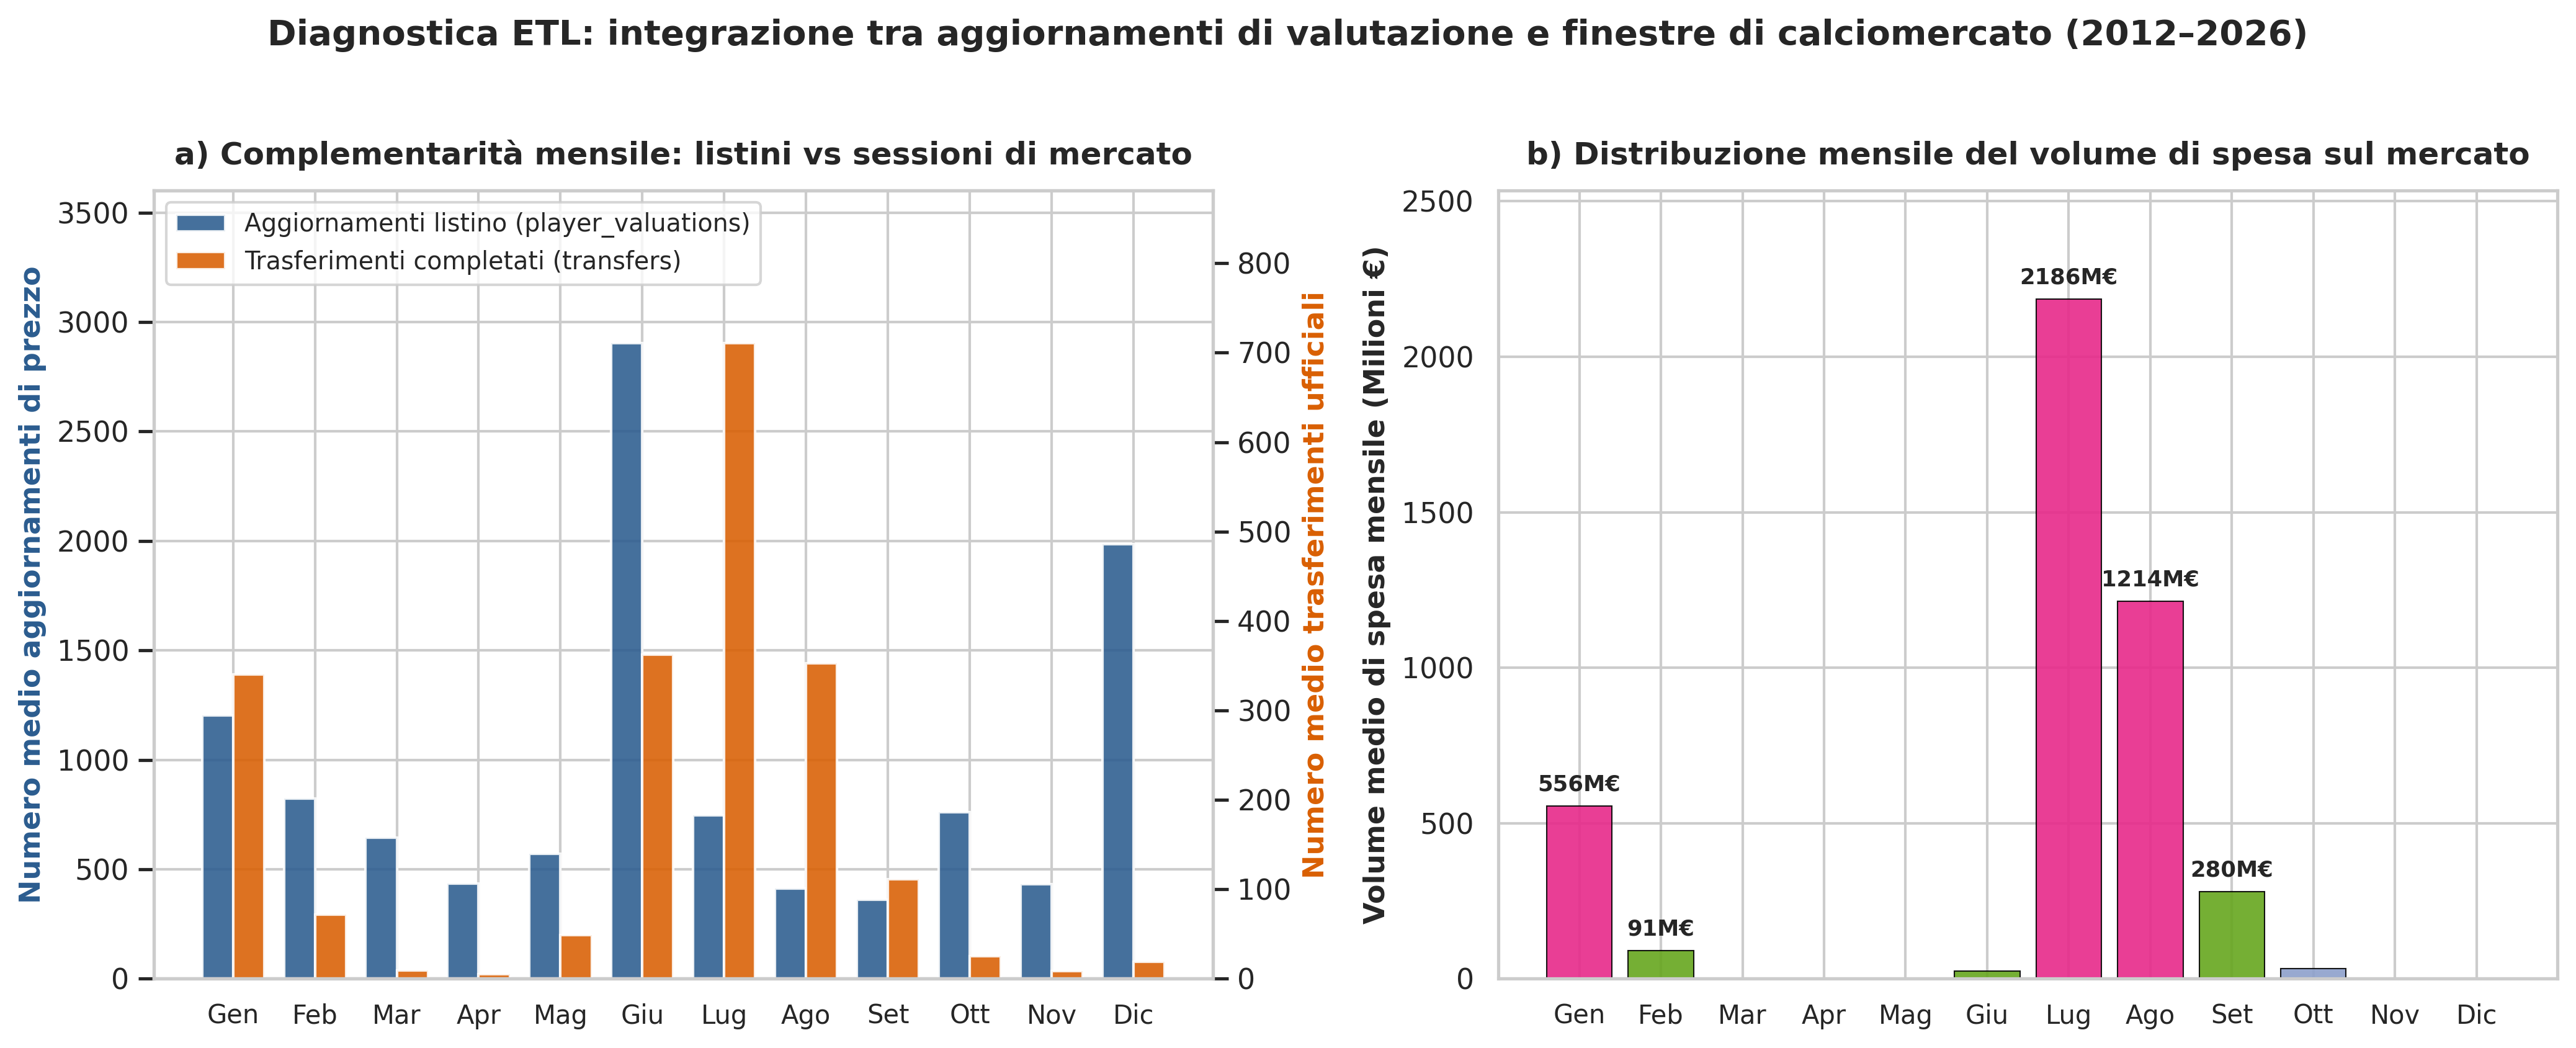
\includegraphics[width=0.98\textwidth]{capitolo6/img/fig01_etl_complementarita_fonti.png}
    \caption{Complementarità stagionale tra la frequenza mensile degli aggiornamenti di valutazione e il volume delle operazioni di calciomercato nei cinque maggiori campionati europei.}
    \label{fig:etl_complementarita}
\end{figure}

Se si aggregassero ingenuamente le sole righe di \texttt{player\_valuations.csv} mese per mese senza mantenere lo stato patrimoniale dei giocatori in attività, la serie risultante rifletterebbe il numero di aggiornamenti redazionali anziché il reale valore delle rose. D'altra parte, se si applicasse una semplice propagazione in avanti delle valutazioni senza tenere conto dei trasferimenti di mercato, la serie presenterebbe dei tratti quasi costanti nei mesi in cui i listini sono fermi.

La seconda criticità riguarda la distorsione retrospettiva legata all'appartenenza dei giocatori ai club. All'interno della tabella \texttt{player\_valuations.csv}, gli attributi \texttt{current\_club\_id} e \texttt{player\_club\_domestic\_competition\_id} non sono variabili storiche indicizzate nel tempo, bensì campi statici che riportano unicamente l'ultima squadra in cui il calciatore milita al momento dell'estrazione del dataset (nel 2026). Di conseguenza, un'aggregazione basata direttamente su tale colonna attribuirebbe l'intera storia passata di un giocatore al suo campionato del 2026: a titolo esemplificativo, atleti protagonisti in Serie A tra il 2018 e il 2021 ma successivamente trasferitisi all'estero (o ritiratisi) non verrebbero conteggiati nel valore storico del campionato italiano, generando una grave sottostima retrospettiva.

Per superare entrambe le problematiche, l'algoritmo di ricostruzione storica implementato nel Listato \ref{lst:etl_ricostruzione} costruisce una griglia temporale mensile regolare (con fase di inizializzazione a partire da gennaio 2009 e finestra di analisi da giugno 2011 a maggio 2026, per un totale di 180 mesi consecutivi pari a quindici cicli annuali completi) ed esegue l'allineamento congiunto dello stato di prezzo e dello stato di appartenenza al club per ciascun giocatore.

\begin{lstlisting}[language=Python, caption={Ricostruzione storica mensile del valore di mercato e del club di appartenenza nello script \texttt{01\_etl\_transfermarkt.py}.}, label={lst:etl_ricostruzione}]
# 1. Griglia mensile regolare e propagazione controllata dell'ultima valutazione valida
grid_months = pd.period_range("2009-01", "2026-05", freq="M")
target_months = pd.period_range("2011-06", "2026-05", freq="M")  # 180 mesi (15 anni)

val_m = vals_sub.groupby(["player_id", "year_month"])["market_value_in_eur"].last().unstack(level=0)
val_ff = val_m.reindex(grid_months).ffill(limit=18)

# 2. Ricostruzione del club storico mese per mese da presenze (appearances) e trasferimenti (transfers)
app_club_m = app_sub.groupby(["player_id", "year_month"])["player_club_id"].last()
tr_club_m = tr_sub.groupby(["player_id", "year_month"])["to_club_id"].last()

club_events = pd.concat([app_club_m, tr_club_m]).groupby(level=[0, 1]).last().unstack(level=0)
club_events = club_events.reindex(index=grid_months, columns=val_ff.columns)
club_hist = club_events.ffill().bfill().fillna(val_club_m)

# 3. Mappatura dal club storico alla rispettiva lega nazionale (IT1, GB1, ES1, L1, FR1)
comp_hist = club_hist.apply(lambda col: col.map(club_to_comp)).fillna("OTHER")
\end{lstlisting}

Come illustrato nel Listato \ref{lst:etl_ricostruzione}, per ogni calciatore e per ciascun mese della griglia temporale viene mantenuta l'ultima valutazione di mercato valida mediante operazione di \textit{forward-fill} limitata a un orizzonte massimo di diciotto mesi, così da garantire la continuità della quotazione per tutti i giocatori in attività ed escludere automaticamente dal computo gli atleti ritirati o inattivi. Contemporaneamente, la matricola del club in cui il giocatore milita in quel preciso mese viene determinata incrociando cronologicamente le presenze effettive in campo tratte da \texttt{appearances.csv} (\texttt{player\_club\_id}) e i cambi di casacca registrati in \texttt{transfers.csv} (\texttt{to\_club\_id}), mappando poi il club storico alla rispettiva competizione nazionale tramite il dizionario estratto da \texttt{clubs.csv}.

L'efficacia di questa ricostruzione ingegneristica è dimostrata visivamente nella Figura \ref{fig:etl_confronto}. Nel pannello superiore viene messo a confronto il valore storico della Serie A ottenuto tramite la nostra ricostruzione dinamica (linea continua verde) con quello prodotto da un'aggregazione statica basata sul solo club del 2026 (linea tratteggiata arancione): quest'ultima sottostima sistematicamente il patrimonio della Serie A lungo tutto il decennio 2014--2022, arrivando a perdere quasi un miliardo di euro di valore reale nel biennio 2019--2020. Al contrario, la serie ricostruita cattura fedelmente sia le acquisizioni internazionali durante le finestre estive e invernali, sia le revisioni periodiche dei cartellini durante il campionato. Nel pannello inferiore della Figura \ref{fig:etl_confronto} è riportata la serie storica principale post-ETL del valore aggregato dei cinque maggiori campionati europei, che evolve in modo continuo da 11,12 miliardi di euro nel giugno 2011 fino al massimo storico di 34,44 miliardi di euro nel maggio 2026.

\begin{figure}[H]
    \centering
    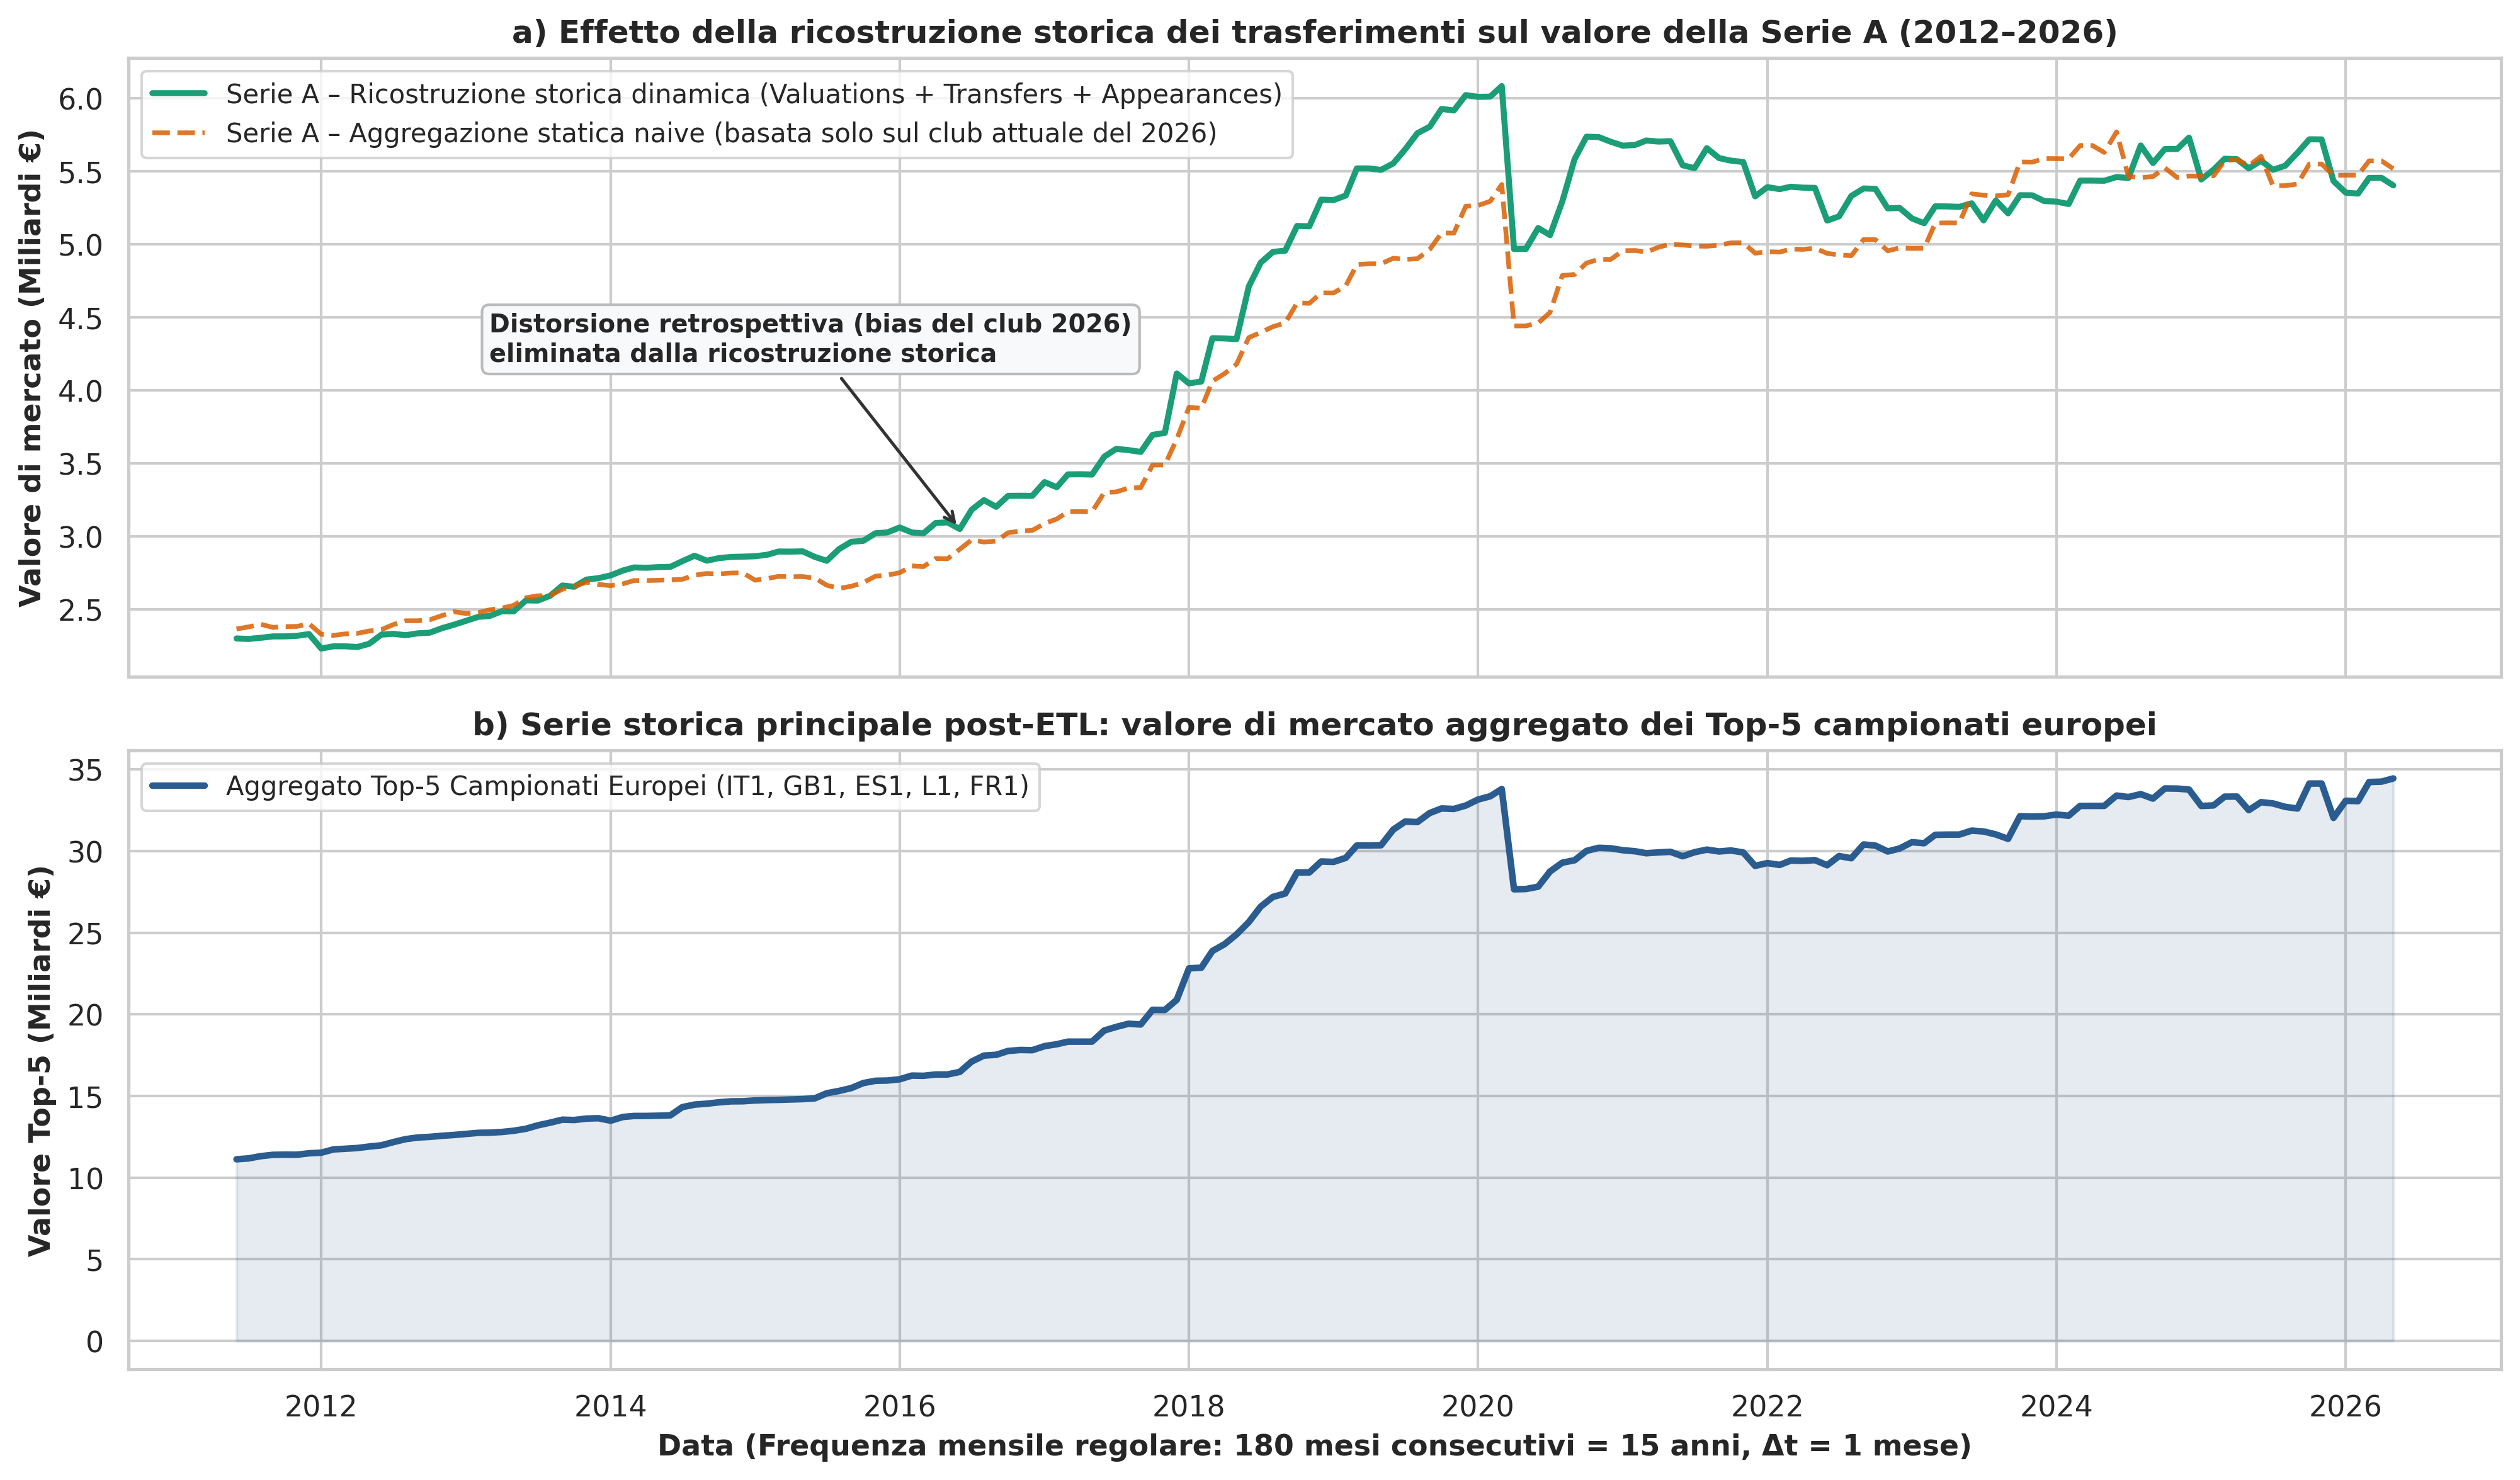
\includegraphics[width=0.98\textwidth]{capitolo6/img/fig02_etl_ricostruzione_storica_confronto.png}
    \caption{Confronto tra aggregazione statica e ricostruzione storica dinamica per la Serie A e andamento complessivo della serie storica principale post-ETL sui 180 mesi di osservazione.}
    \label{fig:etl_confronto}
\end{figure}

La scelta di fissare l'orizzonte temporale definitivo tra giugno 2011 (\texttt{2011-06}) e maggio 2026 (\texttt{2026-05}) risponde a due criteri metodologici rigorosi: da un lato consente di escludere il mese di giugno 2026, parzialmente incompleto nell'estrazione originale e affetto dalla pre-registrazione automatica delle scadenze contrattuali di fine stagione; dall'altro fornisce esattamente 180 osservazioni mensili consecutive, corrispondenti a quindici cicli annuali completi di dodici mesi ($s = 12$). Tale cardinalità permette una suddivisione temporale ottimale per la successiva fase di modellazione predittiva, destinando i primi dodici anni completi (144 mesi, pari all'80\% del campione) al set di addestramento e gli ultimi tre anni completi (36 mesi, pari al 20\%) al set di test.

\begin{table}[H]
\centering
\caption{Struttura delle variabili principali contenute nel dataset mensile elaborato \texttt{market\_monthly.csv}.}
\label{tab:schema_market_monthly}
\begin{tabular}{lll}
\toprule
\textbf{Variabile} & \textbf{Unita / Tipo} & \textbf{Descrizione} \\
\midrule
\texttt{year\_month}, \texttt{date} & Data mensile & Indice temporale regolare ($\Delta t = 1$ mese, 180 osservazioni) \\
\texttt{top5\_market\_value\_bn} & Float (Mld EUR) & Valore di mercato aggregato delle rose dei Top-5 campionati \\
\texttt{serie\_a\_market\_value\_bn} & Float (Mld EUR) & Valore di mercato aggregato delle rose della Serie A (\texttt{IT1}) \\
\texttt{premier\_league\_market\_value\_bn} & Float (Mld EUR) & Valore di mercato aggregato della Premier League (\texttt{GB1}) \\
\texttt{laliga\_market\_value\_bn} & Float (Mld EUR) & Valore di mercato aggregato de LaLiga (\texttt{ES1}) \\
\texttt{bundesliga\_market\_value\_bn} & Float (Mld EUR) & Valore di mercato aggregato della Bundesliga (\texttt{L1}) \\
\texttt{ligue1\_market\_value\_bn} & Float (Mld EUR) & Valore di mercato aggregato della Ligue 1 (\texttt{FR1}) \\
\texttt{mean\_player\_value\_m} & Float (Mln EUR) & Valore di mercato medio per calciatore attivo nei Top-5 \\
\texttt{transfer\_spend\_top5\_m} & Float (Mln EUR) & Volume mensile di spesa per trasferimenti onerosi nei Top-5 \\
\texttt{transfer\_spend\_serie\_a\_m} & Float (Mln EUR) & Volume mensile di spesa per trasferimenti in Serie A \\
\texttt{n\_transfers\_top5} & Intero & Numero totale di trasferimenti completati nel mese \\
\texttt{overpay\_ratio} & Float & Rapporto mediano tra prezzo pagato e valore di mercato \\
\texttt{pct\_change\_top5} & Float (\%) & Variazione percentuale mensile del valore aggregato Top-5 \\
\texttt{shock\_neymar\_post2017} & Binaria [0/1] & Indicatore del regime post-agosto 2017 (shock inflattivo) \\
\texttt{shock\_covid\_2020} & Binaria [0/1] & Indicatore della finestra pandemica e del taglio di aprile 2020 \\
\bottomrule
\end{tabular}
\end{table}

I controlli di integrità eseguiti al termine della pipeline ed esportati nel file di certificazione \texttt{etl\_summary.json} attestano la totale assenza di valori nulli o mesi mancanti (\texttt{missing\_months = 0} su 180 osservazioni) e confermano che la serie principale \texttt{top5\_market\_value\_bn} presenta variazioni non nulle in 179 transizioni mensili consecutive su 179 (\texttt{zero\_change\_months = 0}), soddisfacendo pienamente sia il requisito di equispaziatura temporale sia quello di variabilità dinamica continua. Nella Tabella \ref{tab:schema_market_monthly} vengono infine riassunte le principali variabili salvate all'interno del dataset definitivo \texttt{market\_monthly.csv}, che costituisce la base di partenza per l'analisi esplorativa e la modellazione dei capitoli seguenti.

